In this section, we describe our empirical evaluation of the EAGER
prototype and evaluate its overhead and scaling characteristics.
Figure~\ref{fig:overhead_by_apis} shows that EAGER overhead grows linearly
with the number of APIs exported by an application.  This scaling occurs
because the current prototype implementation iterates through the APIs in the
application sequentially.

\begin{figure}
\centering
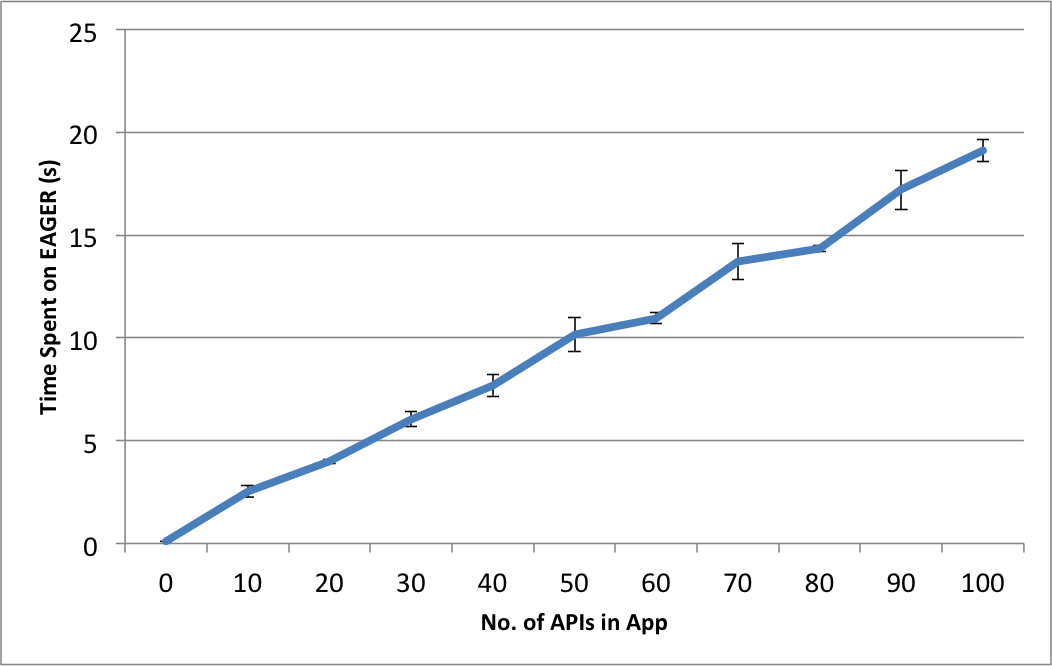
\includegraphics[scale=0.4]{overhead_by_apis}
\vspace{-0.01in}
\caption{EAGER Overhead vs. Number of APIs Exported by the Application}
\label{fig:overhead_by_apis}
%\vspace{-0.1in}
\end{figure}

Next, we analyze EAGER overhead as the number of dependencies declared in
an application grows. For this experiment, we first populate the EAGER
Metadata Manager with metadata for $100$ randomly generated APIs. Then we
deploy an application on EAGER which exports a single API and declares
dependencies on the fictitious 
APIs that are already stored in the Metadata Manager. We
vary the number of declared dependencies and observe the EAGER overhead.

\begin{figure}
\centering
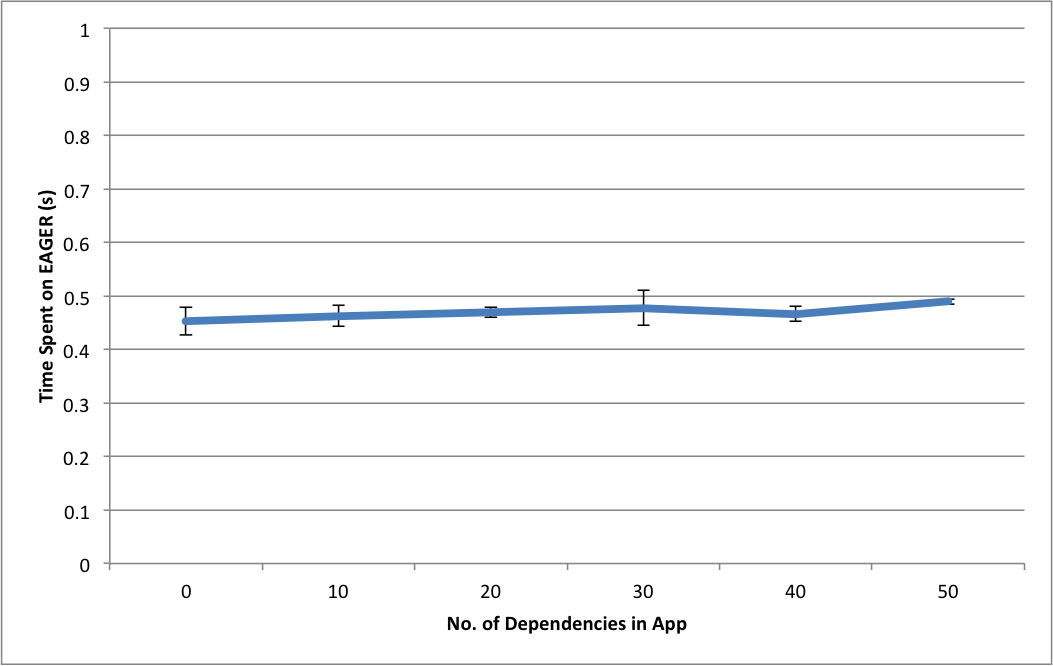
\includegraphics[scale=0.4]{overhead_by_deps}
\vspace{-0.01in}
\caption{EAGER Overhead vs. Number of Dependencies Declared in the Application}
\label{fig:overhead_by_deps}
%\vspace{-0.1in}
\end{figure}

Figure~\ref{fig:overhead_by_deps} shows the results of these experiments. 
EAGER overhead does not appear to be significantly
influenced by the number of dependencies declared in an application. 
In this case, the EAGER implementation processes
all dependency-related information via batch operations. 
As a result, the number of web service calls and database queries that originate 
due to varying number of dependencies is fairly constant. 